\documentclass[tikz,border=3pt]{standalone}
\usepackage{pgfplots}\pgfplotsset{compat=1.18}
\usetikzlibrary{arrows.meta,positioning,calc}
\begin{document}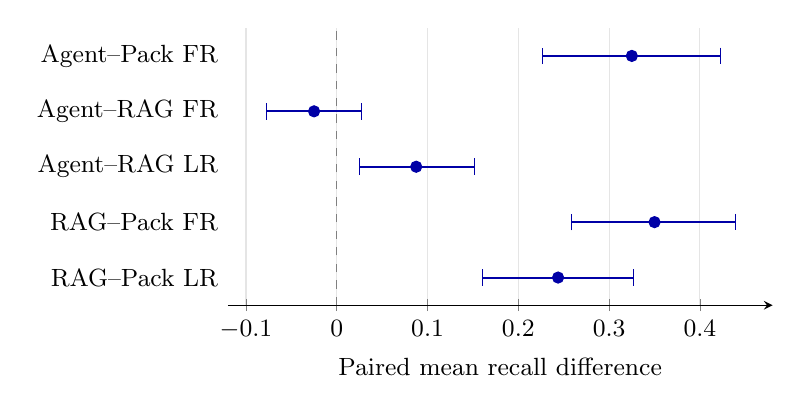
\begin{tikzpicture}
\begin{axis}[width=8.5cm,height=5.1cm,scale only axis=false,
      xmin=-.12,xmax=.48,ymin=-.5,ymax=4.5,
      xlabel={Paired mean recall difference},ytick={0,1,2,3,4},
      yticklabels={RAG--Pack LR,RAG--Pack FR,Agent--RAG LR,Agent--RAG FR,Agent--Pack FR},
      tick label style={font=\small},label style={font=\small},xmajorgrids=true,
      grid style={gray!20},axis y line*=left,y axis line style={draw=none},
      ytick style={draw=none},axis x line=bottom]
      \addplot[gray,dashed] coordinates {(0,-.5) (0,4.5)};
      \addplot+[only marks,mark=*,mark size=2pt,color=blue!65!black,mark options={fill=blue!65!black},
        error bars/.cd,x dir=both,x explicit,error bar style={line width=.7pt},
        error mark options={rotate=90,mark size=3pt}] coordinates {
    (0.325000000000,4) += (0.097916666667,0) -= (0.097916666667,0)
(-0.025000000000,3) += (0.052083333333,0) -= (0.052083333333,0)
(0.087500000000,2) += (0.064583333333,0) -= (0.062500000000,0)
(0.350000000000,1) += (0.089583333333,0) -= (0.091666666667,0)
(0.243750000000,0) += (0.083333333333,0) -= (0.083333333333,0)
};
\end{axis}
\end{tikzpicture}\end{document}
